\documentclass[]{article}
\usepackage[utf8]{inputenc}
\usepackage[english]{babel}
\usepackage{pgfplots}
\pgfplotsset{compat=1.9}
\usepackage{amsfonts}
\usepackage{amsthm}
\newtheorem*{mydef}{Defintion}
\newtheorem*{lemma}{Lemma}

%opening
\title{The Shortcomings of the Field of Constructible Numbers: Generating Field Extensions with Origami}
\author{Jackson Vanover}

\begin{document}

\maketitle

\begin{abstract}
This paper details an exploration of fields and field extensions motivated by the solvability of the classic geometric problem of doubling the cube. The reader will compare and contrast the field of numbers generated by a compass and straightedge combination, call it $E_S$, and the field of numbers generated by paper folding, call it $E_O$. This project involves building up these fields using the axioms for each that determine what are and are not constructible points and lines. In doing so, we will show that $E_0$ is actually a field extension of $E_S$; the reader will see why the solution to the doubling of the cube is not constructible with a compass and straightedge and then how simply folding a piece of paper can solve the problem.
\end{abstract}

\section{Doubling the Cube}
Given a cube with volume $V$, construct a cube with volume $2V$

\section{Essential Definitions}
\begin{mydef}
	A group is a nonempty set with a binary operation, here denoted by juxtaposition, satisfying the following properties:
	\begin{itemize}
		\item Associativity: $(ab)c=a(bc)$,   $\forall a,b,c \in G$
		\item Identity: $\exists e \in G$ such that $ea=ae=a$,   $\forall a \in G$
		\item Inverses: $\forall a \in G$, $\exists a^{-1} \in G$ such that $aa^{-1}=a^{-1}a=e$
		\item Closure: $\forall a,b \in G$, $ab=c \in G$
	\end{itemize}
\end{mydef}
\begin{mydef}
	A group $G$ is abelian if and only if $\forall x,y \in G$, $xy=yx$
\end{mydef}
\begin{mydef}
	A ring is a nonempty set $R$ with two operations, addition and multiplication, satisfying the following properties:
	\begin{itemize}
		\item Under addition, $R$ is an abelian group
		\item Multiplication is associative
		\item Multiplication distributes over addition
	\end{itemize}
\end{mydef}
\begin{mydef}
	A field is a commutative ring (a ring in which multiplication is commutative) in which the subset of nonzero elements forms a group under multiplication.
\end{mydef}
\begin{mydef}
	Let $F$ and $E$ be fields. $E$ is a field extension of $F$ if $F$ is a subfield of $E$, that is to say, all the elements in $F$ are contained in $E$.
\end{mydef}
\begin{mydef}
	$F[x]$ is the set of all polynomials with coefficients in $F$.
\end{mydef}
\begin{mydef}
	Let $E$ be the extension of $F$ containing $\alpha$, a root of some polynomial $f \in F[x]$. Then the field generated by $F$ and $\alpha$, written $F(\alpha)$, is the smallest field extension that contains all the elements of $F$ and $\alpha$.
\end{mydef}
\begin{mydef}
	A real number $r$ is constructible if and only if, given a line segment of unit length, a line segment of length $|r|$ can be constructed.
\end{mydef}

\section{Compass and Straightedge}

\subsection{Construction Axioms} 
\begin{description}
\setlength\itemindent{.5pt}	\item[A1]
	The line through two constructible points is a constructible line
	\item[A2]
	The point of coincidence of two constructible lines is a constructible point
	\item[A3]
	The perpendicular bisector of the segment connecting two constructible points is a constructible line
	\item[A4]
	Given a line that goes through $A$ and $B$, we can construct a line parallel to it through a third given point, $C$
\end{description}

$A1$ and $A2$ are merely statements of fact. We have axiomatized $A3$ and $A4$ for our convenience in later constructions.

\begin{proof}[Proof of Axiom 3:]
	Given a line segment with endpoints $A$ and $B$, start by creating a circle centered at $A$ and going through $B$. Next, create another circle centered at $B$ and going through $A$. These two circles will intersect at two points, $C$ and $D$. The line through $C$ and $D$ is the perpendicular bisector of $AB$
\end{proof}
\begin{proof}[Proof of Axiom 4:]
	Given a line segment with endpoints $A$ and $B$ and a third point, $C$, start by creating a circle centered at $C$ and going through $A$. This circle will intersect segment $AB$ at a point, $E$. By $A3$, construct the perpendicular bisector of segment $AE$ which happens to go through $C$. This line intersects our circle at two points, $F$ and $G$. Construct the line through $F$ and $G$, yielding segment $FG$. By $A3$, find the perpendicular bisector of segment $FG$. This is our parallel line.
\end{proof}

\subsection{Constructing the Ring of Integers}
We begin, by definition, with two points on a plane. We call these points $(0,0)$ and $(1,0)$. Using $A1$, draw the line through these two to construct the real numbers $1$ and $-1$. Note that this line is also our $x$ axis.

Next, create the circle centered at $(1,0)$ and going through $(0,0)$. This circle intersects our $x$ axis at the point $(2,0)$. We have just constructed the real numbers $2$ and $-2$. It is not difficult to see that by repeating this process along the positive $x$ axis, we can construct the ring of integers.

   \begin{figure}[h]
   	\centering
   	\begin{tikzpicture}
   	\begin{axis}[
   	xmin=-1, xmax=4,
   	ymin=-2, ymax=8,
   	axis lines=center,
   	domain=-1:3,
   	xtick=\empty,
   	ytick=\empty,
   	]
   	
   	\addplot [mark=none] {6-3*x};
   	\addplot [mark=none] {3-3*x};
   	\node[label={0:{$B$}},circle,fill,inner sep=2pt] at (axis cs:0,3) {};
   	\node[label={90:{$D$}},circle,fill,inner sep=2pt] at (axis cs:1,0) {};
   	\node[label={0:{$A$}},circle,fill,inner sep=2pt] at (axis cs:0,6) {};
   	\node[label={267.9:{$(1,0)$}},circle,fill,inner sep=2pt] at (axis cs:1,0) {};
   	\node[label={90:{$C$}},circle,fill,inner sep=2pt] at (axis cs:2,0) {};
   	\node[label={150:{$O$}},circle,fill,inner sep=2pt] at (axis cs:0,0) {};
   	\node at (axis cs:1.5,-1) [label={320:{$l1$}},inner sep=0pt] {};
   	\node at (axis cs:2.5,-1) [label={320:{$l2$}},inner sep=0pt] {};
   	\end{axis}
   	\end{tikzpicture}
   	\caption{Division Using Similar Triangles} \label{figure 1}
   \end{figure}
   
\subsection{Constructing the Field of Rational Numbers} 
 In order to proceed, we need to construct  coordinate axes demarcated with the integers. By using $A3$ on the line segment bookended by the points $(-1,0)$ and $(0,0)$, we can construct the $y$ axis. The intersection of the $y$ axis and the circle centered at $(0,0)$ and going through $(1,0)$ will give us the points $(0,1)$ and $(0,-1)$. Then we use the process detailed above to give us the integers along the $y$ axis.
 
  Now, to show that we can construct the field of rationals, we need only show that we can construct any arbitrary rational number of the form $A/B$ where $A,B \in \mathbb{Z}$.
  
  To accomplish this, consider the two constructible points $(0,A)$ and $(0,B)$, corresponding to the two contructible integers, $A$ and $B$ (Refer to {\em Figure 1}). Without loss of generality, let $A>B$. By $A1$, construct the line $l1$ through $B$ and $(1,0)$. By $A4$, construct the line $l2$ parallel to $l1$, thus yielding the constructible point $C$.
   
 Clearly triangles $BOD$ and $AOC$ are similar to one another; by well known properties of similar triangles, we can see that $\frac{OA}{OB}=\frac{OC}{1}=OC$. So, our line segment $OC$ has length $A/B$. This length corresponds to the construction of the rational numbers $A/B$ and $-A/B$. Therefore, we have shown that we can construct the field of the rational numbers using similar triangles.
  
  \begin{figure}[h]
  	\centering
  	\begin{tikzpicture}
  	\begin{axis}[
  	xmin=-6, xmax=3,
  	ymin=-4, ymax=4,
  	axis lines=center,
  	domain=-4:1,
  	xtick=\empty,
  	ytick=\empty,
  	]
  	\node[label={150:{$A$}},circle,fill,inner sep=2pt] at (axis cs:-4,0) {};
  	\node[label={150:{$B$}},circle,fill,inner sep=2pt] at (axis cs:0,0) {};
  	\node[label={45:{$(1,0)$}},circle,fill,inner sep=2pt] at (axis cs:1,0) {};
  	\node[label={45:{$C$}},circle,fill,inner sep=2pt] at (axis cs:0,2.1) {};
  	\node[label={93:{$(\frac{1-a}{2},0)$}},circle,fill,inner sep=2pt] at (axis cs:-3/2,0) {};
  	\end{axis}
  	\draw (3.42,2.83) circle (1.9);
  	\end{tikzpicture}
  	\caption{Construction of Square Roots} \label{figure 2}
  \end{figure}
  
 \subsection{Constructing the Quadratic Closure of the Rationals}
 Let us continue further in our constructions by constructing the square root of a constructible number $a$. (Refer to {\em Figure 2}) Begin with the constructible point $A$ at $(-a,0)$. This point, along with the origin, determines the line segment of length $a$, corresponding to the constructible number $a$. We then create a line segment of length $a+1$ by adjoining the point $(1,0)$ to our segment.
   
 Now, by $A3$, we find the midpoint of this extended line segment, landing at the point $(\frac{1-a}{2},0)$. Construct the circle centered at $(\frac{1-a}{2},0)$ that goes through $A$. This circle will intersect the positive $y$ axis at a point, $C$. The coordinates of $C$ are $(0,\sqrt a)$. Therefore, the segment $BC$ has length $\sqrt a$, corresponding to the constructible numbers $\sqrt{a}$ and $-\sqrt{a}$.

 To see this, evaluate the equation of the circle we constructed at $x=0$.
  
  \[ \bigg(x-\frac{1-a}{2}\bigg)^2 + y^2 = \bigg(\frac{a+1}{2}\bigg)^2 \]
  \[ y^2 = \bigg(\frac{a+1}{2}\bigg)^2 - \bigg((0)-\frac{1-a}{2}\bigg)^2 \] 
  \[ y^2 = \frac{a^2+2a+1}{4} - \frac{a^2-2a+1}{4} \]
  \[ y^2 = a \]
  \[ y = \sqrt{a} \]
  
 So, now we see that the square root of any constructible number is also a constructible number. We have therefore, with a compass and straightedge, constructed a field that is strictly larger than the field of the rational numbers. This field extension of the rational numbers that is closed under square roots (the smallest such extension) is called the \emph{Quadratic Closure of the Rational Numbers}, denote it $\mathbb{Q}^*$.
 
 Note then that both $\mathbb{Q} (\sqrt{2}) \leq \mathbb{Q}^*$ and $\mathbb{Q} (\sqrt{\sqrt{2}}) \leq \mathbb{Q}^*$ since the square root of any constructible number is a constructible number. It is then clear to see that for any $\alpha \in \mathbb{Q}$, $\mathbb{Q} (\alpha ^ \frac{1}{2^n})$ is a subfield of $\mathbb{Q} ^*$.
 
 
  \subsection{Proving $\mathbb{Q}^* = E_S$}
  In order to show that the Quadratic Extension of the Rational Numbers is in fact the set of numbers constructible with a compass and straightedge, recall that, by definition, a constructible number is the length of a constructible line segment. A constructible line segment is defined by two constructible points, let them be $(x_1,y_1)$ and $(x_2,y_2)$, where $x_1,x_2,y_1,y_2 \in \mathbb{Q}^*$. By the distance formula, the constructible real number defined by these points is:
  
 \[z=\sqrt{(x_1-x_2)^2 + (y_1-y_2)^2}\]
  
  Note that due to our premise, $z \in \mathbb{Q}^*$ because $\mathbb{Q}^*$ is a field closed under subtraction, addition, multiplication, and square roots. Therefore, if we wanted to construct a number outside of $\mathbb{Q}^*$, we would need to start with endpoints with components not in $\mathbb{Q}^*$. Let us then look at the three ways in which we construct new points with a compass and straightedge.
  
  First, consider the intersection of two lines:
  
  \[y=m_1 x + b_1\]
  \[y=m_2 x + b_2\]
  
  where $m_1,m_2,b_1,b_2 \in F$ which is some quadratic extension of $\mathbb{Q}$ and a subfield of $\mathbb{Q}^*$. Solving these two linear equations will give us an ordered pair $(\alpha,\beta)$ in which $\alpha,\beta \in F$ because F is a field and is therefore closed under addition, subtraction, multiplication, and division. Therefore, this method will always give us endpoints with components still in $\mathbb{Q}^*$.
  
  Second, consider the intersection of a line and a circle:
  
  \[y=mx+b\]
  \[(x-s)^2 + (y-t)^2 = r^2\]
  
  where $m,b,s,t,r \in F$.
  
  \[x^2-2xs+s^2+(mx+b-t)^2=r^2\]
  \[x^2-2xs+s^2+m^2x^2+2mx(b-t)+(b-t)^2-r^2=0\]
  \[(1+m^2)x^2+(2m(b-t)-2s)x+(s^2+(b-t)^2-r^2)=0\]
  \[x=\frac{-(2m(b-t)-2s)\pm \sqrt{(2m(b-t)-2s)^2-4(1+m^2)(s^2+(b-t)^2-r^2)}}{2(1+m^2)}\]
  \[\Rightarrow x=\frac{-c_2 \pm \sqrt{c_2^2-4(c_1)(c_3)}}{2c_1}\]
  
  where $c_1,c_2,c_3 \in F$ since $m,b,s,t,r \in F$ and F is a field. So, where does $x$ lie? If the discriminant is a perfect square, then we have $x \in F$. If not, then $x$ lies within a quadratic extension of $F$ which is still a subfield of $\mathbb{Q}^*$. In either case, the corresponding $y$ component shares the same field as $x$ since its derivation involves only multiplication by $m \in F$ and addition by $b \in F$. Therefore, this method constructs only points with components in $\mathbb{Q}^*$.
  
  Third and last, consider the intersection of two circles. Notice that this actually amounts to the intersection of a circle and a line, leading us to the same result as above.
  
  So, we can only construct points with entries within the Quadratic Closure of $\mathbb{Q}$, meaning our distance formula will always return a number within the Quadratic Closure of $\mathbb{Q}$. We have therefore shown that $E_S = \mathbb{Q}^*$.
  
  \section{Origami}
  \subsection{Construction Axioms}
  \begin{description}
  	\setlength\itemindent{.5pt}
  	\item[O1]
  	The line connecting two constructible points is a constructible line.
  	\item[O2]
  	The point of coincidence of two constructible lines is a constructible point.
  	\item[O3]
  	The perpendicular bisector of the segment connecting two constructible points is a constructible line.
  	\item[O4]
  	The line bisecting any constructed angle can be constructed.
  	\item[O5]
  	Given a constructed line $l$ and constructed points $P,Q,$ then whenever possible, the line through $Q$, which reflects $P$ onto $l$, can be constructed.
  	\item[O6]
  	Given constructed lines $l,m$ and constructed points $P,Q,$, then whenever possible, any line which simultaneously reflects $P$ onto $l$ and $Q$ onto $m$, can be constructed.
  \end{description}
  	The above axioms all describe the construction of a single fold; the implementation of each is trivial and requires no proof. To these six axioms we will add an incredibly useful Lemma:
    \begin{lemma}
    		Given a point $P$ and a line segment $AB$, we can construct the line through $P$ that is parallel to $AB$
    \end{lemma}
      \begin{proof}
      	By $O1$, connect $P$ to $A$ and $B$, thus creating a triangle. Use $O3$ to construct the midpoint of the three sides of triangle $ABP$; label the midpoints $p,a,$ and $b$, corresponding to the points opposite them. Next, use $O3$ again to construct the midpoint of segment $Pa$, call it $c$. Use $O1$ to construct the line through $A$ and $a$ and the line through $b$ and $c$. These two lines will intersect at a point $D$. Implementing $O1$ with points $P$ and $D$ will give us our parallel line.
      \end{proof}
      
  \subsection{Constructing the Ring of Integers}
  Refer to \emph{Figure 3}. Again, we start with $(0,0)$ and $(1,0)$. $O1$ gives us the $x$ axis and a line segment of length $1$, corresponding to the construction of the integers $1$ and $-1$.
  To proceed with our construction of the ring of integers, we need a $y$ axis. Use $O3$ on our line segment to give us the line $x=\frac{1}{2}$. Our Lemma allows us to construct the line parallel to this going through the origin, yielding our $y$ axis.
  
  Next, we will construct our unit length on the $y$ axis. Use this Lemma again with the point $(1,0)$ to give us the line $x=1$. Then, via $O4$, bisect the right angle formed by $x=1$ and the $x$ axis to get the line $y=1-x$. Its intersection with the $y$ axis gives us the point $(0,1)$.
  
 Using $O4$ to bisect the right angle formed by the $x$ and $y$ axis, construct the line $y=x$. The intersection of $y=x$ and $x=1$ gives us the point $(1,1)$. Using $O1$, construct the line $y=1$. Our Lemma then gives us the ability to construct the line parallel to $y=x$ that goes through the point $(1,0)$, that is, $y=x-1$. The intersection of this line and $y=1$ gives us the point $(2,1)$, from which we can again use the Lemma to construct the line $x=2$ which yields an $x$-intercept of $(2,0)$. We have thus constructed a lines segment of length $2$, corresponding to the construction of the real numbers $2$ and $-2$.
  
  It is not difficult to see that by reiterating this process along the $x$ axis, we can construct the ring of integers. 
   
   \begin{figure}[t]
   	\centering
   	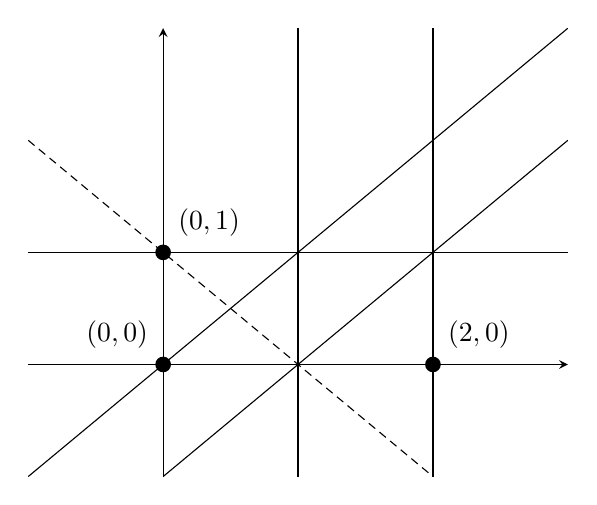
\begin{tikzpicture}
   	\begin{axis}[
   	xmin=-1, xmax=3,
   	ymin=-1, ymax=3,
   	axis lines=center,
   	domain=-1:3,
   	xtick=\empty,
   	ytick=\empty,
   	]
   	
   	\addplot +[mark=none,color=black] coordinates {(1, -1) (1, 3)};
   	\addplot +[mark=none,color=black] coordinates {(-1, -1) (3, 3)};
   	\addplot +[mark=none,color=black] coordinates {(-1, 1) (3, 1)};
   	\addplot +[mark=none,color=black] coordinates {(0, -1) (3, 2)};
   	\addplot +[mark=none,color=black] coordinates {(2, -1) (2, 3)};
   	\addplot +[mark=none,color=black] coordinates {(-1, 2) (2, -1)};
   	\node[label={130:{$(0,0)$}},circle,fill,inner sep=2pt] at (axis cs:0,0) {};
   	\node[label={50:{$(0,1)$}},circle,fill,inner sep=2pt] at (axis cs:0,1) {};
   	\node[label={50:{$(2,0)$}},circle,fill,inner sep=2pt] at (axis cs:2,0) {};
   	\end{axis}
   	\end{tikzpicture}
   	\caption{Constructing the Integers} \label{figure 3}
   \end{figure}
   
   \begin{figure}[t]
   	\centering
   	\begin{tikzpicture}
   	\begin{axis}[
   	xmin=-4, xmax=4,
   	ymin=-5, ymax=2,
   	axis lines=center,
   	domain=-1:3,
   	xtick=\empty,
   	ytick=\empty,
   	]
   	
   	\addplot +[mark=none,color=black] coordinates {(-4, -1) (4, -1)};
   	\addplot +[mark=none,color=black] coordinates {(-.5, -5) (4, 4)};
   	\addplot +[mark=none,color=black,dashed] coordinates {(0, 1) (4, -1)};
   	\node[label={130:{$(0,1)$}},circle,fill,inner sep=2pt] at (axis cs:0,1) {};
   	\node[label={130:{$(0,-a)$}},circle,fill,inner sep=2pt] at (axis cs:0,-4) {};
   	\node[label={10:{$(\sqrt{a},0)$}},circle,fill,inner sep=2pt] at (axis cs:2,0) {};
   	
   	\end{axis}
   	\end{tikzpicture}
   	\caption{Constructing Square Roots} \label{figure 4}
   \end{figure}
  \subsection{Constructing the Field of Rational Numbers}
  Using the power of our Lemma, we can use the exact same process we used with the compass and straightedge using similar triangles to construct any arbitrary rational number.
  
  \subsection{Constructing the Quadratic Closure of the Rationals}
  Let us now show that the square root of any constructible number, $a$, is a constructible number.
  
  Refer to \emph{Figure 4}. Begin with the point $(0,1)$ and the line $y=-1$. Next, consider the point $(0,-a)$, creating a line segment with the origin of length $a$ corresponding to the constructible real number $a$.
  
  By $O5$, construct the line through $(0,-a)$ that reflects $(0,1)$ onto the line $y=-1$.
  
  A quick aside: there is an elegant geometric interpretation of $O5$. The line constructed is the tangent line to the parabola defined by the point being reflected and the line it is being reflected onto, a focus and a directrix respectively. In this example, the parabola in question is $y=\frac{x^2}{4}$.
  
  This newly constructed line will intersect with the $x$ axis at the point $(\sqrt{a},0)$ which, along with the origin, determines a line segment of length $\sqrt{a}$ corresponding to the constructible number $\sqrt{a}$.
  
  How do we see this? We use similar triangles.
  
  Refer to \emph{Figure 5}. Clearly, triangles $OBC$ and $OAC$ are similar. By well known properties of similar triangles and some algebra, we can say the following:
  
  \[\frac{OC}{OB} = \frac{OA}{OC}\]
  \[\frac{OC}{1} = \frac{OA}{OC}\]
  \[OC^2 = OA\]
  \[OC = \sqrt{OA}\]
  
  And segment $OA$ is of length $a$, implying that segment $OC$ is of length $\sqrt{a}$, corresponding to the construction of the real numbers $\sqrt{a}$ and $-\sqrt{a}$.
  
  Therefore, the square root of any constructible number is a constructible number; we have constructed the Quadratic Closure of the Rational numbers with orgiami! So, thus far we have showed that $E_S \subset E_O$.
   \begin{figure}[t]
   	\centering
   	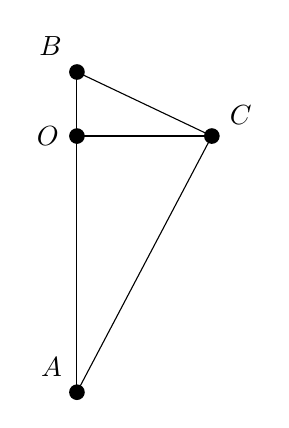
\begin{tikzpicture}
   	\begin{axis}
   	[
   	   	xmin=-4, xmax=4,
   	   	ymin=-5, ymax=2,
   	   	axis lines=none,
   	   	domain=-1:3,
   	   	xtick=\empty,
   	   	ytick=\empty,
   	   	]
   	   	
   	   	\addplot +[mark=none,color=black] coordinates {(0, -4) (0, 1)};
   	   	\addplot +[mark=none,color=black] coordinates {(0, -4) (2, 0)};
   	   	\addplot +[mark=none,color=black] coordinates {(0, 1) (2, 0)};
   	   	\addplot +[mark=none,color=black] coordinates {(0, 0) (2, 0)};
   	   	\node[label={130:{$B$}},circle,fill,inner sep=2pt] at (axis cs:0,1) {};
   	   	\node[label={180:{$O$}},circle,fill,inner sep=2pt] at (axis cs:0,0) {};
   	   	\node[label={130:{$A$}},circle,fill,inner sep=2pt] at (axis cs:0,-4) {};
   	   	\node[label={10:{$C$}},circle,fill,inner sep=2pt] at (axis cs:2,0) {};
   	\end{axis}
   	\end{tikzpicture}
   	\caption{Similar Triangles} \label{figure 5}
   \end{figure}
   
  \subsection{Constructing Cube Roots}
  Notice then that we have not yet used $O6$. We will use this last axiom to show that the cube root of any constructible number is a constructible number. We do this by showing that we can construct a line segment of length $\sqrt[3]{a}$ where $a$ is a constructible number.
  
  Refer to \emph{Figure 6}. Begin with the same focus and directrix as in the previous section, $(0,1)$ and $y=-1$ respectively. Next, construct a second focus and directrix at $(-a,0)$ and $x=a$.
  
  Implement $O6$, which is actually just two simultaneous implementations of $O5$, to construct the line that reflects both $(0,1)$ onto $y=-1$ and $(-a,0)$ onto $x=a$. Similar to $O5$, the geometric interpretation of this fold is the creation of a single line that is tangent to both of the parabolas defined by our two sets of foci and directrices.
  
  This tangent line intersects the $x$ axis at the point $(\sqrt[3]{a},0)$. We prove this again using similar triangles. We will adopt the notation and conclusions from the previous section.
  
     \begin{figure}[t]
     	\centering
     	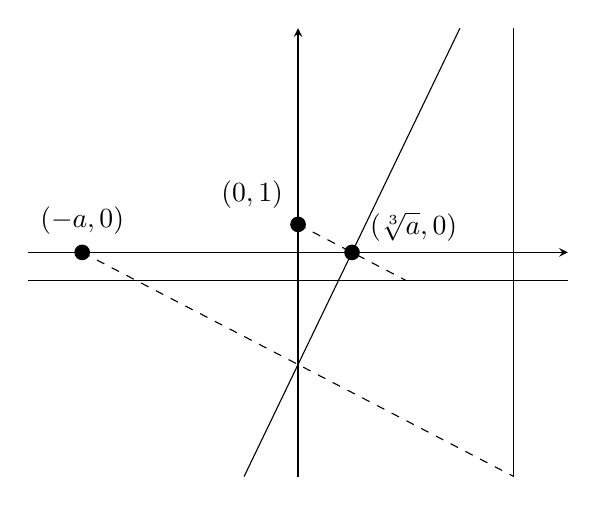
\begin{tikzpicture}
     	\begin{axis}[
     	xmin=-10, xmax=10,
     	ymin=-8, ymax=8,
     	axis lines=center,
     	domain=-1:3,
     	xtick=\empty,
     	ytick=\empty,
     	]
     	
     	\addplot +[mark=none,color=black] coordinates {(-10, -1) (10, -1)};
     	\addplot +[mark=none,color=black] coordinates {(8, -8) (8, 8)};
     	\addplot +[mark=none,color=black] coordinates {(-2, -8) (6, 8)};
     	\addplot +[mark=none,color=black,dashed] coordinates {(0, 1) (4, -1)};
     	\addplot +[mark=none,color=black,dashed] coordinates {(-8, 0) (8, -8)};
     	\node[label={130:{$(0,1)$}},circle,fill,inner sep=2pt] at (axis cs:0,1) {};
     	\node[label={90:{$(-a,0)$}},circle,fill,inner sep=2pt] at (axis cs:-8,0) {};
     	\node[label={10:{$(\sqrt[3]{a},0)$}},circle,fill,inner sep=2pt] at (axis cs:2,0) {};
     	
     	\end{axis}
     	\end{tikzpicture}
     	\caption{Constructing Cube Roots} \label{figure 6}
     \end{figure}
     
        \begin{figure}[t]
        	\centering
        	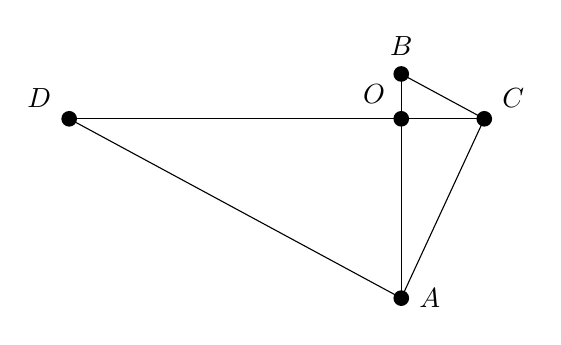
\begin{tikzpicture}
        	\begin{axis}
        	[
        	xmin=-9, xmax=4,
        	ymin=-5, ymax=5,
        	axis lines=none,
        	domain=-1:3,
        	xtick=\empty,
        	ytick=\empty,
        	]
        	
        	\addplot +[mark=none,color=black] coordinates {(0, -4) (0, 1)};
        	\addplot +[mark=none,color=black] coordinates {(0, -4) (2, 0)};
        	\addplot +[mark=none,color=black] coordinates {(0, 1) (2, 0)};
        	\addplot +[mark=none,color=black] coordinates {(-8, 0) (2, 0)};
        	\addplot +[mark=none,color=black] coordinates {(-8, 0) (0, -4)};
        	\node[label={90:{$B$}},circle,fill,inner sep=2pt] at (axis cs:0,1) {};
        	\node[label={140:{$O$}},circle,fill,inner sep=2pt] at (axis cs:0,0) {};
        	\node[label={0:{$A$}},circle,fill,inner sep=2pt] at (axis cs:0,-4) {};
        	\node[label={10:{$C$}},circle,fill,inner sep=2pt] at (axis cs:2,0) {};
        	\node[label={170:{$D$}},circle,fill,inner sep=2pt] at (axis cs:-8,0) {};
        	\end{axis}
        	\end{tikzpicture}
        	\caption{Similar Triangles} \label{figure 7}
        \end{figure}
        
    
    Refer to \emph{Figure 7}. We start by recognizing that triangle $OAD$ and triangle $OBC$ are similar. We can then do the following:
    
    \[\frac{OC}{OB}=\frac{OD}{OA}\]
    \[\frac{OC}{1}=\frac{OD}{OA}\]
    \[(OC)(OA)=OD\]
    
    Recall that our prior calculations with similar triangles gave us $OC^2=OA$. Substituting this in, we get:
    
    \[OC^3=OD\]
    \[OC=\sqrt[3]{OD}\]
    
    By our construction, line segment $OD$ is of length $a$, indicating that segment $OC$ is of length $\sqrt[3]{a}$, corresponding to the construction of the real numbers $\sqrt[3]{a}$ and $-\sqrt[3]{a}$ Therefore, the cube root of any constructible number is also a constructible number!
    
    We have therefore shown that the set of origami constructible numbers is in fact strictly larger than the Quadratic Closure of the Rationals and furthermore, we now know that $E_S \subset E_O$. To be more specific, $E_O$ is a field extension of $E_S$ that allows for closure under cube roots.
    
    \section{Solvability of the Doubling of the Cube}
    So what does constructing the solution to the Doubling of the Cube look like? Recall that we are given a cube of volume $V$ from which we must construct a cube with volume $2V$.
    
    Let the side lengths of our original cube be $l$. This implies that $V=l^3$. We then have that $2V=2l^3$ from which it follows that the side lengths of our new cube must be $l\sqrt[3]{2}$.
    
    We know that $l$ is constructible because our original cube has side lengths $l$. The question then lies in whether or not $\sqrt[3]{2}$ is constructible. To use the notation introduced in Section 2, we want to know if $\mathbb{Q}(\sqrt[3]{2}) \subset E_S$ or if $\mathbb{Q}(\sqrt[3]{2}) \subset E_O$.
    
    From our constructions above, we have shown that $E_S$ is not closed under cube roots, but $E_O$ is. Therefore, $\mathbb{Q}(\sqrt[3]{2}) \not\subset E_S$ and $\mathbb{Q}(\sqrt[3]{2}) \subset E_O$. $\sqrt[3]{2}$ is constructible with origami but not with compass and straightedge, indicating the solvability of the problem of doubling the cube in the case of the former mode of construction but not the latter.
    
    \section{Further Origami Constructions}
    Notice that we have not showed that $E_O$ is strictly limited to the field extension of $E_S$ that allows for closure under cube roots. The potential for origami constructions extends much further, and an exploration of all of its applications is beyond the scope of this paper. However, one such application that may surprise is the constructibility of the solutions to quintic equations.
    
    Now, it is important to note that the axioms we have described for origami constructions (owed to the work of Jacques Justin, Humiaki Huzita, Koshiro Hatori, and Robert Lang) describe the creation of \emph{single} folds. Utilizing just these axioms, quintic equations are in fact unsolvable using paper folding. However, it is possible to define axioms that allow for the simultaneous creation of \emph{multiple} folds that cannot be decomposed into the composition of our original six axioms. These non-separable folds make up a new class of origami construction axioms which have the potential to solve equations of much higher order, like fifth-order polynomials.
    
    For further information on this, the reader is directed toward Alperin and Lang's paper entitled \emph{One-, Two-, and Multi-Fold Origami Axioms}.
    
    \section*{References}
    \begin{description}
    	\item[[ 1]]
    	Roger Alperin, \emph{A Mathematical Theory of Origami Construction and Numbers}
    	\item[[ 2]]
    	Winston Gao, \emph{Field Extensions and the Classical Compass and Straight-Edge Constructions}
    	\item[[ 3]]
    	James King, \emph{Origami Constructible Numbers}
    	\item[[ 4]]
    	Roger Alperin and Robert Lang, \emph{One-, Two-, and Multi-Fold Origami Axioms}
    \end{description}
\end{document}